\documentclass[floatfix, apj]{emulateapj}

% latex ms.tex; bibtex ms; latex ms; latex ms; dvips ms; ps2pdf ms.ps ; gv ms.pdf
% latex ms.tex; bibtex ms; latex ms; latex ms; dvips ms; ps2pdf ms.ps ; open ms.pdf
\usepackage[paperwidth=8.5in, paperheight=11in, centering, margin=1in]{geometry}
\usepackage{amsmath}
\usepackage{epsfig}

\def\aap{{\it Astr.~Ap.}}     %Astronomy & Astrophysics%
\def\aaps{{\it A\&AS}}
\def\apj{{\it ApJ}}

\begin{document}
\title{Regularization Techniques for PSF--Matching Kernels. II. Pre--Filtering Input Images}

\author{
A.C.~Becker\altaffilmark{1},
R.H.~Lupton\altaffilmark{2},
K.S.~Krughoff\altaffilmark{1},
et al.
}
\altaffiltext{1}{Astronomy Department, University of Washington, Seattle, WA 98195}
\altaffiltext{2}{Department of Astrophysical Sciences, Princeton University, Princeton, NJ 08544}

\date{\today}

\begin{abstract}

We report on a novel technique for reducing the numbers of false detections in difference images due to deconvolution (or sharpening) by the profile--matching kernel.
In this technique, we pre--smooth the input science image by its own point spread function before performing profile--matching.
This results in a maximum--likelihood image for point source detection, which has a $\sqrt{2}$ broader point--source profile than the original image PSF.
We then match a reference image to this smoothed image, effectively resulting in a point--source maximum likelihood difference image.
The process of detection happens directly on this difference image; however, measurement techniques must be modified to operate on such a PSF--smoothed image.
By smoothing the input image, we reduce the number of conditions under which the reference image has to be sharpened to match the input image, which is a significant source of systematic false detections.
We note that this technique commutes with the traditional order of operations, in which two images are PSF--matched, then then filtered for detection by the science image PSF.
We compare these two techniques by measuring the empirical rates of false detections in a suite of high--fidelity simulated images from the Large Synoptic Survey Telescope (LSST).
We additionally compare the empirical rates to those expected from random fluctuations in the background Gaussian field, including the run of false positives with detection threshold.
In order for there to be less than 1 expected false detection per LSST sensor, the detection pipeline must operate at a threshold of 5.5--sigma under median (0.6'') seeing conditions.
%
In the traditional post--filtering process, deconvolution leads to a significant number of false detections at high signal--to--noise, while also resulting in a loss of sensitivity for true variability.
In post--filtering and pre--filtering convolutions, we find a close match in the number of false detections versus detection threshold, when performing a 1--parameter correction to the effective detection threshold to account for misestimation of the image noise.
The image variance is shown to be underestimated by approximately 1\% in the pre--filtering detection image, and at a similar amount in the post--filtering difference image.
However, when smoothing the post--filtering difference image for detection, the image variance becomes significantly overestimated under the deconvolution conditions, and overestimated by approximaetely 4\% under convolution conditions.
This suggests that the multiple integral transforms being applied to images lead to significant misestimations of the variance, as the pixels become correlated and current algorithms do not track the pixel covariance during these operations.
Our study shows that even a 2\% misestimate of the noise may change the false detection rate by a factor of 1.5--2 at the 5--sigma detection threshold.
We also find that over or under--subtraction of the image background leads to a bias in the positive--going to negative--going false detection ratio, but not on the overall number of detections.
%
We describe a set of testing protocols to tune the configuration of the overall PSF--matching algorithm and to compare techniques.
For a given set of data, the pipeline is configured to minimize the mean--squared--error of a control sample of sources not used in the matching kernel fit.
To compare techniques, we use the use the total number of false detections that are associated with sources in the image to study systematic errors, and ``orphan'' detections to study sensitivity to statistical fluctuations.
Our simulated image suite allows us to control the ground truth behind the images, which is invaluable in understanding the nature of the false detections.
\end{abstract}
\keywords{methods: data analysis, techniques: image processing}

\section{Introduction}

Image subtraction as a solution to general crowded--field variability detection.
PSF-matching as a means to image subtraction.
Sources of false detections (in binary classification these would be naturally referred to as ``false positives''.  However, since ``positive'' also may refer to the polarity of a difference image detection, and we indeed accept both positive--going and negative--going detections as ``false positives'', we choose to use the term ``false detections'' here to refer to these systematic errors).
Machine learning as a way to address false positive rate.
LSST.
Alert stream.
Mention that one paper that talks about pre--filtering but not for this reason.

\section{PSF--Matching Algorithm}

We outline the image subtraction process below.
We assume that science image $S(x,y)$ can be modeled as a convolution of the template image $T(x,y)$ by a PSF--matching kernel $K(u,v;x,y)$ (indices $u,v$ indicate that the kernel itself is a 2--dimensional function, which varies as a function of position $x,y$ in the image.
During convolution and correlation there is an implicit summation over $u,v$).
The two images will have different point spread functions (PSFs), which are the time--averaged transfer functions of a point source through the Earth's atmosphere, telescope optics, and into the silicon of the detector before being read out.
The essence of image subtraction is to match the PSFs of these two images so that they may be subtracted pixel by pixel.

We further assume that the PSF--matching kernel may be decomposed using a set of basis functions $K(u,v) = \sum_i a_i K_i(u,v)$, where the coefficients in front of each basis are determined through:
\begin{eqnarray}
\label{eq-soln}
C_i & \equiv & (K_i \otimes T) \\ 
b_{i}  & = & \sum_{x,y} {{C_i(x,y) S(x,y)}\over{\sigma^2(x,y)}}   \nonumber \\
M_{ij} & = & \sum_{x,y} {{C_i(x,y) C_j(x,y)}\over{\sigma^2(x,y)}}  \nonumber \\
a_{i}  & = & M^{-1}_{ij} b_{j} \nonumber
\end{eqnarray}
Here $\sigma^2(x,y)$ is the per--pixel variance.
To generate a spatially varying model for the kernel, we assume that the relative weights of the basis functions $a_i$ themselves vary spatially, i.e. $K(u,v;x,y) = \sum_i a_i(x,y) K_i(u,v)$.
In general, one may assume that there is a differential background between the two images $b(x,y)$ that may be fit for using a low--order polynomial.
The image difference is then calculated through $D(x,y) = S(x,y) - T(x,y) \otimes K(u,v;x,y) - b(x,y)$.

The basis functions themselves $K_i(u,v)$ are a degree of freedom in this problem.
The original implementations \citep{Alard98,Alard00} used a set of 3 Gaussians, each with a different width, and each modified by a Laguerre polynomial to a given order.
Subsequent studies \citep[e.g.][]{2007AN....328...16I} have suggested that a constant ratio be maintained between the different Gaussian widths, such that $\sigma_{i+1} = \beta \times \sigma_{i}$.
We use the value $\beta = 2.0$ here.
We set the overall scale for sigma by noting that, under the assumption that the PSFs of the images are Gaussian ($\sigma_S$ for the science image and $\sigma_T$ for the template image), the sigma of the matching kernel should be simply $\sigma_K^2 = \sigma_S^2 - \sigma_T^2$.
We use this width for the central Gaussian in a 3--component basis, with the smaller/larger Gaussian a factor of $1/\beta$ and $\beta$ different, respectively.

Detection on the difference image occurs after correlation of $D(x,y)$ with the science image's PSF, yielding optimally--filtered detection image $D'(x,y) = D(x,y) \circ PSF_S(u,v;x,y)$, where the $\circ$ operator denotes correlation.
The values of the pixels in $D'(x,y)$ provide a maximum likelihood estimate of there being a point source at that position.
Detection occurs by finding single pixels in $D'(x,y)$ that are more than N sigma above the square root of the per--pixel background variance.

In this work we investigated two orders of operations for the optimal filtering by the PSF.
In the first method, which is the classical post--filtering implementation of the technique, we create a difference image that is then post--filtered with the PSF for detection:
\begin{eqnarray}
D_{Post}(x,y) & = & S(x,y) - T(x,y) \otimes K(u,v;x,y)  \nonumber \\
D'_{Post}(x,y) & = & D_{Post}(x,y) \circ PSF_S(u,v;x,y).  \nonumber
\end{eqnarray}
In the second method, which we refer to as pre--filtering, we match the template image to a PSF--filtered science image:
\begin{eqnarray}
D_{Pre}(x,y)  & = & S(x,y) \circ PSF_S(u,v;x,y) - \nonumber \\ 
             &   & T(x,y) \otimes K(u,v;x,y) \nonumber \\
D'_{Pre}(x,y) & = & D_{Pre}(x,y). \nonumber
\end{eqnarray}
By pre--smoothing the image that we are matching the template to -- $S(x,y) \circ PSF_S(u,v;x,y)$ -- we increase the effective point--source profile width by a factor of $\sqrt{2}$.
This allows for less frequent {\it deconvolution} of the template image, or when the template FWHM is larger than the FWHM in the image it is being matched to.
We are able to run detection directly on $D_{Pre}(x,y)$, but measurement requires a modified suite of algorithms.

\section{Input Data}

In order to test the efficacy of these two algorithms, we generated simulated images using the LSST PhoSim package v3.2.5 \cite{phosim}.
These images are high--fidelity simulations of the end--to--end LSST system, including effects from the atmosphere, optics, and detectors.
In order to establish a algorithmic baseline, we turned off certain confounding elements of the simulations, including airglow variations, cloud screens, tracking variations, quantum efficiency variations, diffraction, saturation, and blooming.
An input stellar catalog was generated to seed the simulation that included a random field with of $1000$ stars per sensor, and an equivalent $r$-band magnitude range ($19<r<21$).
All stars in the sample had identical spectral energy distributions, corresponding to a Kurucz--model XXX star \cite{kurucz}, to avoid chromatic effects.
For these sources, proper motion, parallax, and variability were set to zero.
Thus there is no intrinsic variability of any sort designed into the simulated images, and any detections in their difference will be by--definition false positives.

Each simulation run was generated using the following configurations:
\begin{itemize}
\item {\tt Visit 0}: A 300s template image with an atmospheric seeing value of 0.88 arcsec.
\item {\tt Visit 1}: A 15s science image with 0.6 arcsec atmospheric seeing.
\item {\tt Visit 2}: A 15s science image with 0.88 arcsec atmospheric seeing.
\item {\tt Visit 3}: A 15s science image with 1.2 arcsec atmospheric seeing.
\end{itemize}
The seeing of the template image was designed to result in a sharpening deconvolution when compared to {\tt Visit 1}, and a smoothing convolution when compared to {\tt Visit 3}.
All observations were simulated at the zenith, and all images were simulated in the $i$--band.
Sky backgrounds in the resulting images were at the level of $\sim 150$ counts per pixel.
Nine sensors of the central raft were simulated, for a total of 27 difference images per configuration (9 sensors each with 3 seeings to compare to the template image) to use in our comparative analysis.

\section{Optimizing the Algorithm}

To assess the ``quality'' of each implementation of the algorithm, we use as a metric the number of false positive--going and negative--going sources that are detected and measured in each difference image.  We describe our image processing pipeline below, and then describe our assessment and tuning of difference image quality.

% Once we found an optimum configuration, we perturbed the solution along multiple dimensions to understand how the false detection rate responded.

\subsection{Pipeline Implementation}

At the start of the pipeline, we have a pair of template and science images that we wish to astrometrically and photometrically register.
The process of astrometric registration refers to the exact alignment of the two images in pixel space, while photometric alignment refers to matching of the PSF shape, sky backgrounds, and zero--point.
From the input reference catalog we choose 80\% of the stars to use in the registration process, with the remaining 20\% of the objects serving as a control sample to assess
the effectiveness of $K(u,v;x,y)$ to subtract objects that were {\it not} used in the fits.
A direct image--to--image relative astrometric mapping was determined using the detected sources in the template and science images, and a sinc--based resampling kernel applied to the template image (as it has larger signal--to--noise than the science image).
The resulting warped image was used as the image subtraction template $T(x,y)$.
The science image $S(x,y)$ (optionally pre-filtered with its $PSF_S(u,v;x,y)$) and $T(x,y)$ were sent to the image subtraction task, whose purpose is to fit for $K(u,v;x,y)$ and to produce the difference image $D(x,y)$.

The first step in this process is to use the PSF Gaussian widths to define the {\it sizes} of the Gaussians' shapes in $K_i(u,v)$.
It is important to note that these widths are {\it not} configurable within the PSF--matching, and must be chosen by the user beforehand.
As mentioned above, the central Gaussian width was chosen to be $\sqrt{\sigma_S^2 - \sigma_T^2}$, and smaller and larger Gaussians used that were scaled a factor of $\beta = 2$.
We modified each of the Gaussians by a set of Laguerre polynomials of a given order.
The smallest Gaussian was modified to the specified order, with the others modified by floor(order/2).
For the process of deconvolution, we followed the prescription from \cite{0266-5611-26-8-085002} to choose basis shapes.
In our implementation of this algorithm, the number of Gaussians is {\it always} fixed to value 3, and their Laguerre degree is always fixed to 3.
The  widths of the Gaussians are determined through the algorithm specified in \cite{0266-5611-26-8-085002}, using as inputs the sequence of Gaussians that we would have used to match a Gaussian of
  width $\sigma_S$ to $\sigma_T$ (i.e. as if we would have convolved the science image and not the template image).
The total number of basis shapes in each set is: $\sum_i^{\rm nGauss} ({\rm degGauss}_i+1)\times({\rm degGauss}_i+2)/2$.

As in the astrometric resampling, we choose to always perform pixel--level operations on the template image given its larger signal--to--noise, and (in the case of real data) fewer artifacts such as dead pixels and cosmic rays.
The dimensions of the PSF matching kernel were chosen to be 6 times the largest Gaussian width, with a minimum kernel size of 21x21 pixels.
For kernels that are significantly smaller than this, the Gaussians have significant (non--zero) power at the kernel boundaries, leading to square systematic artifacts at the scale of the kernel in the difference images.

For each source indexed by $j$, we create substamps from each image $T_j(x,y)$ and $S_j(x,y)$ centered on the source.
These were used to fit for a local solution $K_j(u,v)$; the ensemble of local solutions at each source's $x,y$ was used to fit for the full spatial solution $K(u,v;x,y)$.
We emphasize that the dimensions of the substamps are important.
Note from Equation~\ref{eq-soln} that $C_i$, and thus the coefficients $a_i$, are derived from a convolution of the template substamp with the kernel basis functions $K_i$.
This convolution means that kernel size//2 pixels along the border of each substamp are rendered unusable.
To maintain a significant number of pixels in $C_i$, we set the stamp dimensions to be twice that of the kernel dimensions, such that the number of pixels remaining in $C_i$ is equal to the number of pixels in the kernel.

For each source, we solved for $K_j(u,v)$ to create a local difference image $D_j(x,y)$.
We evaluated several statistics on this local difference image, normalized by the square root of its variance, which puts the pixels in units of $\sigma$.
We measured the mean sigma, the RMS of this distribution, the $\chi^2$ of these pixels normalized by the degrees of freedom (number of pixels in $D_j(x,y)$ minus the number of kernel bases), and the mean squared error.
These are referred to as the {\tt LOCAL} kernel metrics, and reflect how appropriate the chosen kernel basis is.

The ensemble of sources was then used to constrain a spatial model of the kernel $K(u,v;x,y)$.
For the spatial kernel model, we assumed that each of the kernel coefficients $a_i$ may be represented by a $N^{th}$ order 2--dimensional Chebyshev polynomial.
Having generated the full spatial solution $K(u,v;x,y) = \sum_i a_i(x,y) K_i(u,v)$, we evaluated the spatial kernel solution at the position of each source, created a new difference image using this kernel, and recalculated the metrics defined above.
These are referred to as the {\tt SPATIAL} kernel metrics.
Importantly, we also interpolated this solution to the positions of the control sample, which were explicitly {\it not} used in the spatial fit, and evaluated these same metrics.
The differences between the {\tt LOCAL} and {\tt SPATIAL} metrics, as well as the values of the {\tt SPATIAL} metrics for the control sample, reflect the appropriateness of the spatial model and our ability to interpolate and extrapolate to the full extent of the images.
We used the Mean Square Error (MSE) of the control sample to examine the tradeoff between bias and variance in the spatial interpolation.
We define the bias as $\left| data - model \right|$, the variance as $(data - model)^2$, and the MSE as {\tt bias$^2$ + variance}.  
In this context, the bias is the mean of the difference image, and the variance is the mean square of the difference image.
We found that N = 5 or 6 was sufficient to minimize the control sample MSE, or maximize the predictive power of the spatial model without overfitting.

Figure~\ref{fig:1} presents 4 sets of common image subtraction failure modes, and associated poor choices in pipeline configuration that may cause them.

\begin{figure*}[!ht]
  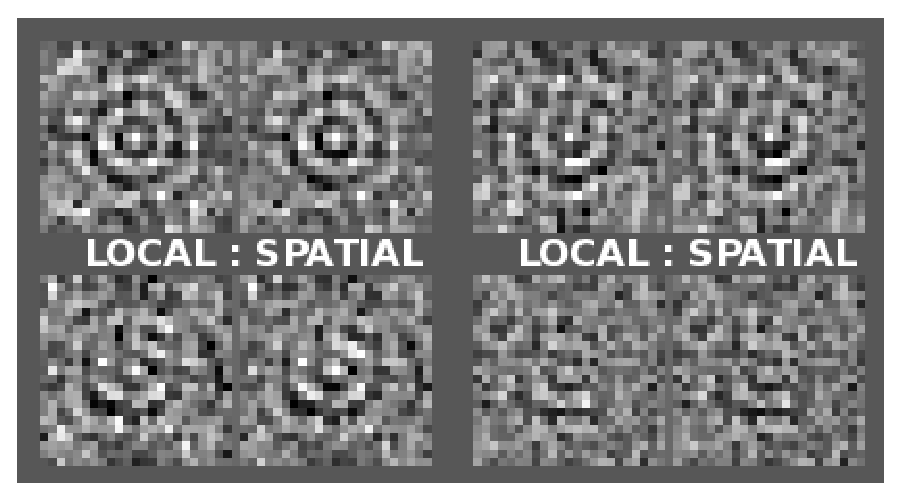
\includegraphics[width=0.5\textwidth, height=0.25\textwidth]{fig1a.eps}
  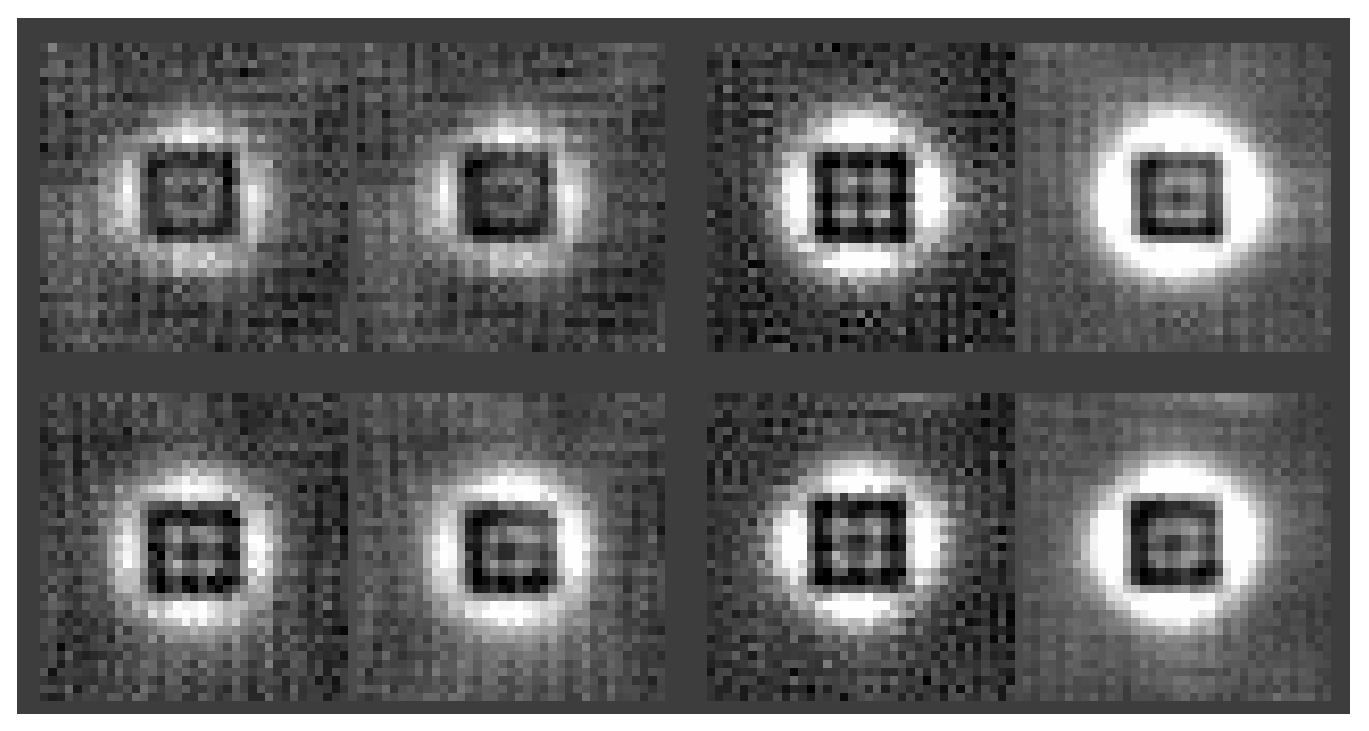
\includegraphics[width=0.5\textwidth, height=0.25\textwidth]{fig1b.eps} \\
  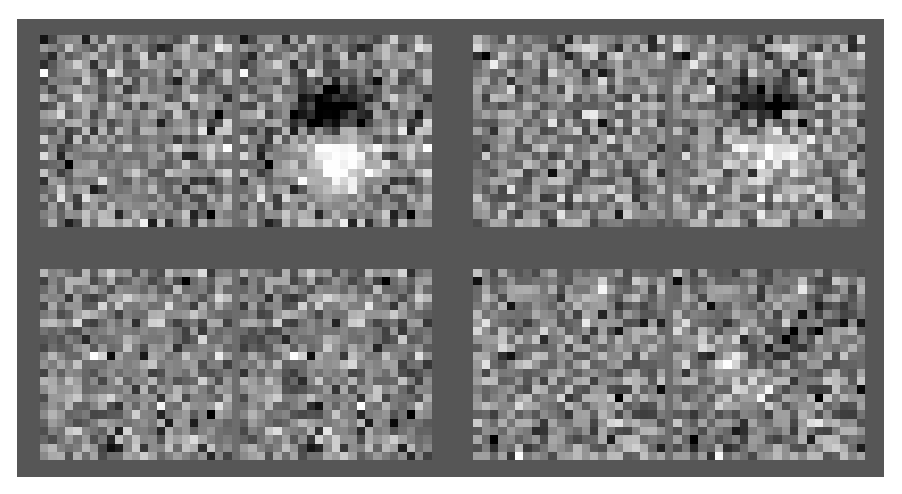
\includegraphics[width=0.5\textwidth, height=0.25\textwidth]{fig1c.eps}
  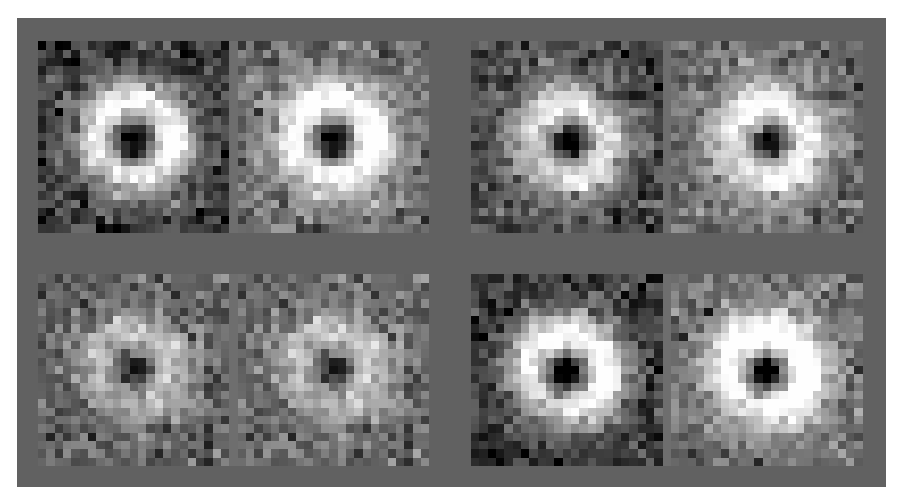
\includegraphics[width=0.5\textwidth, height=0.25\textwidth]{fig1d.eps} \\
\caption{Four example panels showing failure modes of the image
  subtraction software.
  Each panel itself shows a 2x2 pair of difference images; on the {\it
    left} subpanel is the residual from the {\tt LOCAL} fitting, and
  on the {\it right} from the {\tt SPATIAL} fitting.
  Starting in the upper left and proceeding clockwise, the first panel
  shows the residuals when deconvolving the template image; the
  ringing in both solutions is characteristic of the deconvolution
  process.
  Upper right, a set of difference images where the kernel dimensions
  (kernel size) are too small given the widths of the Gaussians, such
  that the value of the kernel does not fall to zero along its
  boundary.
  This leaves square kernel--sized residuals around each object.
  Lower right, a set of images where the kernel shape (Gaussian sigma) is
  inappropriate to match the sources; note that the {\tt LOCAL}
  residuals also show circular residuals, indicating the basis set
  itself is at fault (as opposed to the spatial model).
  Finally, in the lower left, a set of images that demonstrate how the
  residuals degrade when the spatial kernel model is at fault.
  Note that the {\tt LOCAL} residuals appear to be white noise, while
  the {\tt SPATIAL} residuals show a clear dipole signature.
  For this reason, a comparison between the {\tt LOCAL} and {\tt
    SPATIAL} residuals is a useful diagnostic of the spatial model.
  The dipoles may also arise due to problems in the astrometric
  remapping (e.g. too low an order), or for individual extreme--color
  objects objects due to differential chromatic refraction.
}
\label{fig:1}
\end{figure*}


\subsection{Source Detection}

We next perform the process of source detection on the full difference images.
In post--filtering, we convolved the difference image with its PSF (by design, the same as the PSF of $S$) before detection.
In the case of pre--filtering, we detected on the difference image directly.
We looked for both positive and negative--polarity detections, and performed the detection step at several significance thresholds to understand the the numbers of false detections at each significance level.
These detections were merged together (e.g. to join the positive and negative lobes of a dipole) using a grow radius of 2 pixels.

Since the fundamental image operations are the same, the images immediately preceding the detection step ($D'$) should have been {\it exactly} the same.
As we will demonstrate in Section~\ref{sec-uh}, this was not exactly the case.

All difference image sources (henceforth diaSources) were associated with the reference catalog, with a matching radius of 3''.
We used this association to help assess if the diaSource was a source--associated false detection that came from the image subtraction software, or an orphan statistical fluctuation in the background.

\subsection{Source Measurement}

We outline the process of point--source PSF--weighted flux measurement below.
We start with the definition of PSF--weighted flux assuming a normalized PSF, $PSF$:
%
\[F_j = \frac{\sum_{(x,y)}S_j(x,y) * PSF_j(x,y)}{\sum_{(x,y)}PSF_j^2(x,y)}\]
%
where $S_j(x,y)$ is the image before PSF filtering, and $PSF_j^(x,y)$ is an image of the PSF centered on the source.
This equation assumes an isolated point source in a background--subtracted image.

We note that the convolution of an entire image $S(x,y)$ by its spatially varying $PSF(u,v;x,y)$, when evaluated at a single pixel, corresponds to multiplying the PSF matrix with a similarly sized matrix of pixels from the source image, centered on the source of interest.  Thus the PSF--weighted flux in a post--filtered difference image $D$ is 
%
\[F_{Post,j} = \frac{\sum_{(x,y)}D_{Post}(x,y) * PSF_j(x,y)}{\sum_{(x,y)}PSF_j^2(x,y)}\]
while the flux in a pre--filtered difference image $D'$ is simply
\[F_{Pre,j} = \frac{D_{Pre}(x,y)}{\sum_{(x,y)}PSF_j^2(x,y)}.\]

We further define
%
\[w(x,y) \equiv \frac{PSF(x,y)}{\sum_{(x,y)}PSF^2(x,y)}.\]
%
To calculate the variance in the measurement, we assume a point source model for the intensity:
%
\[S(x,y) = A * PSF(x,y) + \epsilon(x,y)\]
\[\langle F \rangle = \langle \sum_{(x,y)} w(x,y)(A * PSF(x,y) +\epsilon(x,y))\rangle\]
%
with a scaling factor $A$ and white noise contribution $\epsilon(x,y)$.
Since $\langle \epsilon(x,y) \rangle = 0$ and $\langle \epsilon(x,y) * \epsilon(x',y') \rangle = \sigma^2(x,y)\delta(x-x', y-y')$:
%
\[\langle F \rangle = \sum_{(x,y)} w(x,y) * A * PSF(x,y)\]
and
\[\sigma^2_F \equiv \langle(F - \langle F \rangle)^2\rangle,\]
such that
\[\sigma^2_F = \frac{\sum_{(x,y)}PSF^2(x,y)\sigma^2(x,y)}{(\sum_{(x,y)} PSF^2(x,y))^2}.\]
This implies that the error $\sigma_{F}$ on the flux at location x,y is a weighted sum of the per--pixel variance in the input image.

The center of each source is determined using an LSST adaptation of the SDSS centroiding algorithm \cite{photo}.
In general a source will not be centered on a pixel, so a Lanczos resampling kernel is used to shift the source to be centered on the nearest pixel before applying the measurement equations above.

\section{False Detection Rate}

We examine our realized false detection rate, both in comparison to the theoretical statistical floor, and as intercomparison between the post and pre--filtering techniques.

\subsection{Theoretical \label{sec-analyticfp}}

We model a source--free image (i.e.\ with a background described by a Gaussian process) using the statistics of Gaussian random fields \citep{Kaiser-PointSources}.
For an image with Gaussian noise convolved with a Gaussian PSF with width $\sigma_g$, the density of peaks above a given detection threshold $\nu$ is given by
\begin{equation}
n(>\nu) = \frac{1}{2^{5/2}\pi^{3/2}} \nu e^{-\nu^2 /2}.
\label{eq-theory}
\end{equation}
To estimate the number of random positive detections for a given image we must normalize this density by the total number of realizations of the PSF within the image, i.e.,
\begin{equation}
N_{total}(>\nu) = n(>\nu)*nrow*ncol/ \sigma_g^2
\label{eq-theorytot}
\end{equation}
where $nrow$ and $ncol$ are the number of image rows and columns.
In difference image analysis, we expect twice this number, since we are sensitive to both positive and negative--going fluctuations.
We created an empty sky--only simulated image, and recorded the number of detections in this image as a function of threshold.
This showed good agreement with twice the amount indicated by Equation~\ref{eq-theorytot}, indicating that the simulated background is well described by a random Gaussian field.

Table~\ref{tab-fp} lists shows the number of false detections {\it per sensor} for an LSST--sized device, as a function of detection threshold.
We used a Monte Carlo approach to estimate the variance on the predicted false detection rate as a function of threshold, using $10^6$ realizations, to provide the uncertainties on the column values.
Note that to reduce the number of false positives to less than 1 per sensor, under 0.6'' seeing conditions, the detection threshold should be set at a minimum of 5.5 sigma.
This value might indeed be allowed to float with seeing, such that the survey would make itself more sensitive to lower S/N objects under worse seeing conditions.

\begin{table*}[t]
\centering
\begin{tabular}{ccccc}
\hline
\multicolumn{5}{|c|}{Theoretical Number of False Detections per Sensor} \\
\hline
Visit    & FWHM (pixels) & $\sigma=4.5$ & $\sigma=5.0$ & $\sigma=5.5$\\
\hline
{\tt 1} & 3.0 & 114$\pm$11 & 12$\pm$3& 1$\pm$1\\
{\tt 2} & 4.4 & 54$\pm$8 & 5$\pm$2& 0.5$\pm$0.5\\
{\tt 3} & 6.0 & 29$\pm$6 & 3$\pm$2&0.2$\pm$0.4\\
\end{tabular}
\caption{{\rm Total number of false detections that we expect based on a
  4000x4072 pixel sensor.  This number is dependent on the seeing and
  detection threshold, so we list the values at a threshold of 4.5,
  5.0, and 5.5 sigma for the seeings in the 3 visits used in this
  study.  We list the total number of positive {\it plus} negative
  detections, which should be present in equal quantities. The variance
  is determined through Monte Carlo simulation.\label{tab-fp}}}
\end{table*}

\subsection{Empirical}

We report here the results for each of the 3 visits, and for pre-- and post--filtering for detection, using our optimal pipeline configuration.
We use measurement flags to remove spurious detections on the immediate border of the image; other than that we do no other cuts other than requiring that the centroid measurement is finite, which would be a realistic requirement for any real--time alert system reporting on these objects.
We separated the diaSources that match with the reference catalog (using a 3'' matching radius) from those that don't (referred to as orphans) to investigate the origins of the detections.
We found no significant correlation of false detections rate with sensor within the raft; therefore we report the aggregate results for all 9 sensors in the analyses that follow.

\begin{table*}[t]
\centering
\begin{tabular}{clc|ccccc}
\hline
\multicolumn{8}{|c|}{False Detection Counts} \\
\hline
Visit   & Filtering & N$_{Expect}$ & N$_{Measured}$ &  N$_{Orphan}$ & N$_{Match}$ & N$_{Random}$ & N$_{-}$ / N$_{+}$\\
\hline
{\tt 1} & Pre      & 108$\pm$27   & 70      &60         & 10 & 3  & 1.8 \\ 
        & Post     & $\cdots$     & 143     &51         & 92 & 2  & 0.4 \\
{\tt 2} & Pre      & 45$\pm$18    & 42      &36         & 6  & 2  & 2.6 \\
        & Post     & $\cdots$     & 53      &45         & 8  & 2  & 0.5 \\
{\tt 3} & Pre      & 27$\pm$18    & 23      &23         & 0  & 1  & 2.8 \\
        & Post     & $\cdots$     & 36      &35         & 1  & 1  & 3.4 \\
\end{tabular}
\caption{Total number of diaSources detected at 5--sigma from all 9 sensors in raft 2,2 (N$_{Measured}$).
  N$_{Expect}$ lists the total number we expect to detect as random fluctuations, from Table~\ref{tab-fp}, and are the same for pre and post--filtering.
  Whether a detection is a match (N$_{Match}$) or an orphan (N$_{Orphan}$) is determined using a 3'' match radius with the input reference catalog.
  We list the number of background fluctuations that are expected to randomly associate with a Source N$_{Random}$, given the density of objects in the images and a 3'' match radius, assuming that N$_{Orphan}$ represents 96\% of the total population of detections from Gaussian fluctuations.
  \label{tab-bestfp10}}
\end{table*}

The numbers N$_{Measured}$ of false detections in each best case are given in Table~\ref{tab-bestfp10}, with the total number expected from the Monte Carlo analysis given as N$_{Expect}$.
We undertook a manual inspection of all difference images to associate the diaSources with sources in the images, ultimately using a 3'' association with the input source catalog to formally define matches and orphans.
Associations are listed in the N$_{Match}$ column of Table~\ref{tab-bestfp10}, with the unmatched false positives in the N$_{Orphan}$ column.
The former are likely to come from systematics in the subtractions of stars, while the latter would be due to fluctuations in the background.
We note two effects that may impact N$_{Match}$.
The first is that, with a 3'' matching radius and our source densities, 4\% of random fluctuations will by--chance associate with a source.
Assuming that N$_{Orphan}$ represents 96\% of the background fluctuation population, we estimate the number of fluctuations from that same population that would have associated with sources as N$_{Random}$.
We note that there is a slightly higher number of associations with sources than we would expect randomly (N$_{Random}$ $<$ N$_{Match}$), although this is rare and at the rate of 1 every 4--5 images.
In the last column of Table~\ref{tab-bestfp10} we list the ratio of negatively detected to positively detected diaSources.

\section{Sources of False Detections}
We examine in detail the sources of the false detections in these images.
This includes an investigation of the sky subtraction in the images, how knowlwedge of the image noise impacts the false detection rate, and the run of false positives with detetion threshold.

\subsection{Sky subtraction}

The ratio of negative to positive diaSources is significantly higher than 1.0 for all pre--filtering visits.
We examine modeling of the sky background as a potential source for this systematic.
The top panel of Figure~\ref{fig:2} shows contours of positive to negative false detections, overlayed on a sky backgorund over or under--subtraction vs. detection threshold plot.
We find that, at a 5--sigma detection treshold, a 1.5\% sky misestimate can bias the ratio of positive to negative sources by a factor of 2.
The bottom panel shows contours of the {\it total} numbers of false detections, positive plus negative, and we see that this value is relatively insensitive to the sky model.
As more detections of one polarity are found, fewer of the other are found, although the bias is to slowly increase the total numbers of false detections.
The observed ratios of 2--3 suggest that there is a background overestimation of order $1-2\%$ causing lower--sigma fluctuations to be measured at 5--sigma (Figure~\ref{fig:2}).
\begin{figure*}[!ht]
\centering
\centering{\includegraphics[width=1.0\textwidth]{fig2.eps}}
\caption{
Misestimation of the sky background value has an effect on both the number of false detections, and relative abundance of positive to negative false detections.
The top pane of this figure shows the relative number of +ve/-ve (-ve/+ve) detections if the sky background is under (over) subtracted at a particular fractional level.
The  bottom panel shows how the total number of false detections changes for the same misestimation.
This is not a strong function of the seeing; these numbers are appropriate for the 0.6'' simulation presented here.
}
\label{fig:2}
\end{figure*}

\subsection{Image Variance \label{sec-varmis}}

Figure \ref{fig:3} shows the effect of misestimating the noise in the detections for each of three different seeing values (0.6$^{\prime\prime}$, 0.88$^{\prime\prime}$, 1.2$^{\prime\prime}$ respectively).
In each case the top panel shows the number of additional expected false positives in an LSST--sized CCD, given a fractional misestimation of the noise in the image and a detection threshold.
A 1\% {\it under}--estimate of the noise corresponds to ~4 additional false positives at a threshold of $5\sigma$ in the best seeing case, compared to 12 expected (Table~\ref{tab-fp}), and 1 additional false positive in the worst seeing case, compared to 3 expected.
These additional numbers roughly double if the noise is underestimated by 2\%.
The bottom panels show the effect of {\it over}--estimating the noise in the measurement; as expected, the effect is to reduce the number of false positives.
A 1\% under-estimate of the noise typically results in 2 fewer false positives per chip, at 5--sigma.
\begin{figure*}[!ht]
  \includegraphics[width=0.33\textwidth]{fig3a.eps}
  \includegraphics[width=0.33\textwidth]{fig3b.eps}
  \includegraphics[width=0.33\textwidth]{fig3c.eps} \\
  \caption[]{ We plot here the expected change in the total number of
    false detections as a function of detection threshold and noise
    misestimate.
    The panels on these 3 pages are for three values of seeing,
    left--to--right 0.6'', 0.88'', 1.2''.
    In each panel the top pane shows the rate increase when the noise
    is under--estimated, and the bottom shows the rate decrease when
    the noise is over--estimated.
    In all cases the counts are for the total number of false
    positives in a single 4000x4072--pixel random Gaussian field.
  }
  \label{fig:3}
\end{figure*} 

\subsubsection{Comparison of Empirical vs. Proposagated Noise Properties}


%{\bf good point: note that the curves nfp vs. threshold are
%  correlated, its a cumulative distribution}.

Since these images will have gone through multiple convolutions before reaching the detection stage, it is expected that the propagated per--pixel variance will not provide an exact representation of the empirical variance in the image planes \citep{Price-Stacking}.
Because the astrometric resampling uses a warping kernel that is designed to preserve the noise properties of the images, we expect that the kernel convolution will provide the largest sources of such error.

To quantify this, we first compared the empirical variance in the image planes with the level tracked by the variance planes, for images $D$ and $D'$.  
We calculated the ratio of the interquartile range of unmasked pixels in the image plane, multiplied by 0.741 and then squared, with the median of unmasked pixels from the variance plane.  
The former represents the empirical variance, while the latter the propagated variance.  
We investigate their ratio (empirical/propagated) at 2 stages in the processing: after creation of the difference image (image $D$), and immediately preceding detection (image $D'$).  
Recall that for pre--filtering, $D = D'$.  
These results are summarized in Table~\ref{tab-variance1}.  
For pre--filtering, we find that the variance plane typically underestimates the true variance by $1\%$ for all visits.  
When using post--filtering, the deconvolution {\tt Visit 1} yields a similar underestimate in the difference image, but for the other two visits the variance is tracked to better than 1\%, with a small RMS.  
However, when post--filtering with the PSF, the variance becomes {\it overestimated} by nearly a factor of two for deconvolution {\tt Visit 1}, and {\it underestimated} by $4-5\%$ for the other visits.
This will yield a smaller number of false detections during deconvolution, and a larger number of false detections during convolutions.

\begin{table*}[t]
\centering
\begin{tabular}{clccc}
\hline
\multicolumn{4}{|c|}{Variance Ratios: Empirical / Propagated} \\
\hline
Visit    & $D_{pre} = D'_{pre}$ & $D_{post}$ & $D'_{post}$ \\
\hline
v6866601 &$1.012 \pm 0.002$&$1.018 \pm 0.005$&$0.599 \pm 0.017$ \\
v6866602 &$1.010 \pm 0.002$&$1.007 \pm 0.001$&$1.046 \pm 0.002$ \\
v6866603 &$1.015 \pm 0.003$&$1.008 \pm 0.001$&$1.045 \pm 0.003$ \\
\end{tabular}
\caption{Ratio of the empirical variance in the difference images,
  calculated using the square of (0.741 times the interquartile range), to the
  median of the variance plane.
  In all cases (except the deconvolution configuration) the variance plane
  represents an {\it underestimate} of the true variance in the
  images.
  We report the mean and RMS across all sensors.
}
\label{tab-variance1}
\end{table*}

\subsubsection{Investigating the Asymmetry Between Pre and Post--Filtering}

We next investigated the variance properties of the images that are input to the detection stage, i.e. the difference image itself in the case of pre--filtering, and the difference image convolved with its PSF in post--filtering.
These results are summarized in Table~\ref{tab-variance2}.
We find that the image planes have very similar empirical noise properties at the detection stage, with the deconvolution visit having larger variance by $1\%$ but the other visits having essentially equal noise properties, with a bias towards the post--filtered data having slightly higher variance (while the RMS is small, all values are greater than 1.0)\footnote{For completeness, we note the median differences between the image planes at the time of detection are 3--4 counts (or 0.2 sigma relative to the empirical variance) for v6866601, 0.2 counts (0.02 sigma) for v6866602, and less than 0.1 counts (0.01 sigma) for v6866603.}.
The medians of the variance planes tell a different story though.
For the deconvolution visit, the median per--pixel variance is $70\%$ higher.
While this will suppress the detections of false positives, it will also significantly suppress the detection efficiency for true variability.
For the other visits, the post--filtered per--pixel variance is relatively {\it lower} by $3-4\%$.
This will increase the sensitivity of the post--filtered data to false positives; as shown in Table~\ref{tab-bestfp10}, the rate is indeed larger using the post--filtering pipeline.
This analysis demonstrates that this is primarily due to an {\it underestimate} of the per--pixel variance in the post--filter processing: while the pre--filtered variance is a 1\% underestimate, the post--filtered variance is a 5\% underestimate.
As outlined by \cite{Price-Stacking}, this is due, at least in part, to loss of pixel covariance when undergoing multiple convolutions, as covariance is not currently tracked in the LSST software used here.
In pre--filtering, the science image undergoes a single convolution, and the template image a single convolution.
In post--filtering, the template image undergoes a convolution, is subtracted from the science image, and then undergoes a second convolution with the Psf.
As we have demonstrated here, this second convolution is where our variance bookkeeping lags the empirical variance.

\begin{table*}[t]
\centering
\begin{tabular}{ccc}
\hline
\multicolumn{3}{|c|}{Variance Ratios: $D'_{post} / D'_{pre}$} \\
\hline
Visit    & Empirical & Propagated \\
\hline
v6866601 & $1.011 \pm 0.016$    & $1.710 \pm 0.049$    \\
v6866602 & $1.001 \pm 0.001$    & $0.967 \pm 0.001$    \\
v6866603 & $1.002 \pm 0.001$    & $0.974 \pm 0.002$    \\
\end{tabular}
\caption{Ratios of the variance planes immediately before detection
  $D'$.
  Ratios are in the sense of the variance of the post--filtered
  image divided by the variance of the pre--filtered image.
  The first
  column represents the ratios of the empirical variance, calculated
  via the square of (0.741 times the interquartile range).
  The second column
  reports the ratios of the medians of the propagated variance planes.
  We report the mean and RMS across all sensors.}
\label{tab-variance2}
\end{table*}


\subsection{Detection Threshold}
Obviously the number of false positives will be strongly dependent on the detection threshold.
In order to check the scaling of false detection rates with threshold, we ran the detection and measurement pipelines using several detection threshold values.
As discussed in Section~\ref{sec-analyticfp} one can predict the number of false detections expected in a sensor given seeing and threshold values.
The top row of Figure~\ref{fig:4} shows the results of this analysis.
From left to right the panels are for {\tt Visit 1} (0.6$^{\prime\prime}$ FWHM), {\tt Visit 2} (0.88$^{\prime\prime}$ FWHM) and {\tt Visit 3} (1.2$^{\prime\prime}$ FWHM) respectively.
We show the theoretical run of false detections vs. threshold in black, with a 1--sigma envelope coming from Monte Carlo simulations (Section~\ref{sec-analyticfp}).
The red squares show the empirical rates coming from the classical post--filtering analsis, while the blue circles are for the pre--filtering technique presented here.
It is noteworthy that the deconvolution configuration shows an enhanced number of false positives at high significance.
Since our analysis shows that we should be {\it less} sensitive to false detections in deconvolution, these should most prominently be coming from systematic mis--subtraction of source in the image.
These features typically appear as ringing in the images around bright sources, which trigger the detection algorithm.
As seen in Table~\ref{tab-bestfp10}, there are indeed an enhanced number of false positives that match to an image source (92 out of 143).
This demonstrates that the deconvolution process results in higher sensitivity to systematic features, and lower sensitivity to real fluctuations.

Also of note is that the majority of the curves lie {\it below} the theoretical expectations, although within the uncertainties.
This is not entirely unexpected, as each curve is strongly correlated, being a cumulative distribution, and represents only 9 samplings of the background random Gaussian field.
However, it may also signify a systemic issue in the analyses applied to these images.
Since our analysis indicates that the total number of false detections are realtivly insensitive to background subtraction issues, but strongly sensitive to varience estimation,
we explore a 1--parameter correction to the effective detection threshold to see if we can bring our data in--line with expectations.
Specifically, we define scaling factor $k$ to correct the counts at a given threshold:
\begin{equation}
n_{corrected}(>\nu) = n(> k * \nu)
\label{correction}
\end{equation}

The bottom panel of Figure~\ref{fig:4} shows the results of this correction, using $k = 0.975, 0.985 $~and~$ 0.99$ for {\tt Visit 1}, {\tt Visit 2}, and {\tt Visit 3}, respectively
These results suggest our variance estimates are too {\it high}, and we are therefore detecting too {\it few} false detections.
This does not agree entirely with the analysis of the empirical variance, Section~\ref{sec-varmis} and Table~\ref{tab-variance1}, which suggest that our variance planes {\it underestimate} the true variance.
However, this makes clear that while we are at the level of the theoretical floor in false detection rate, it is imperative to track the variance in our data at the 1\% level or better to optimize both the false detection rate, and the true detection efficiency.
\begin{figure*}[!ht]
  \centering
  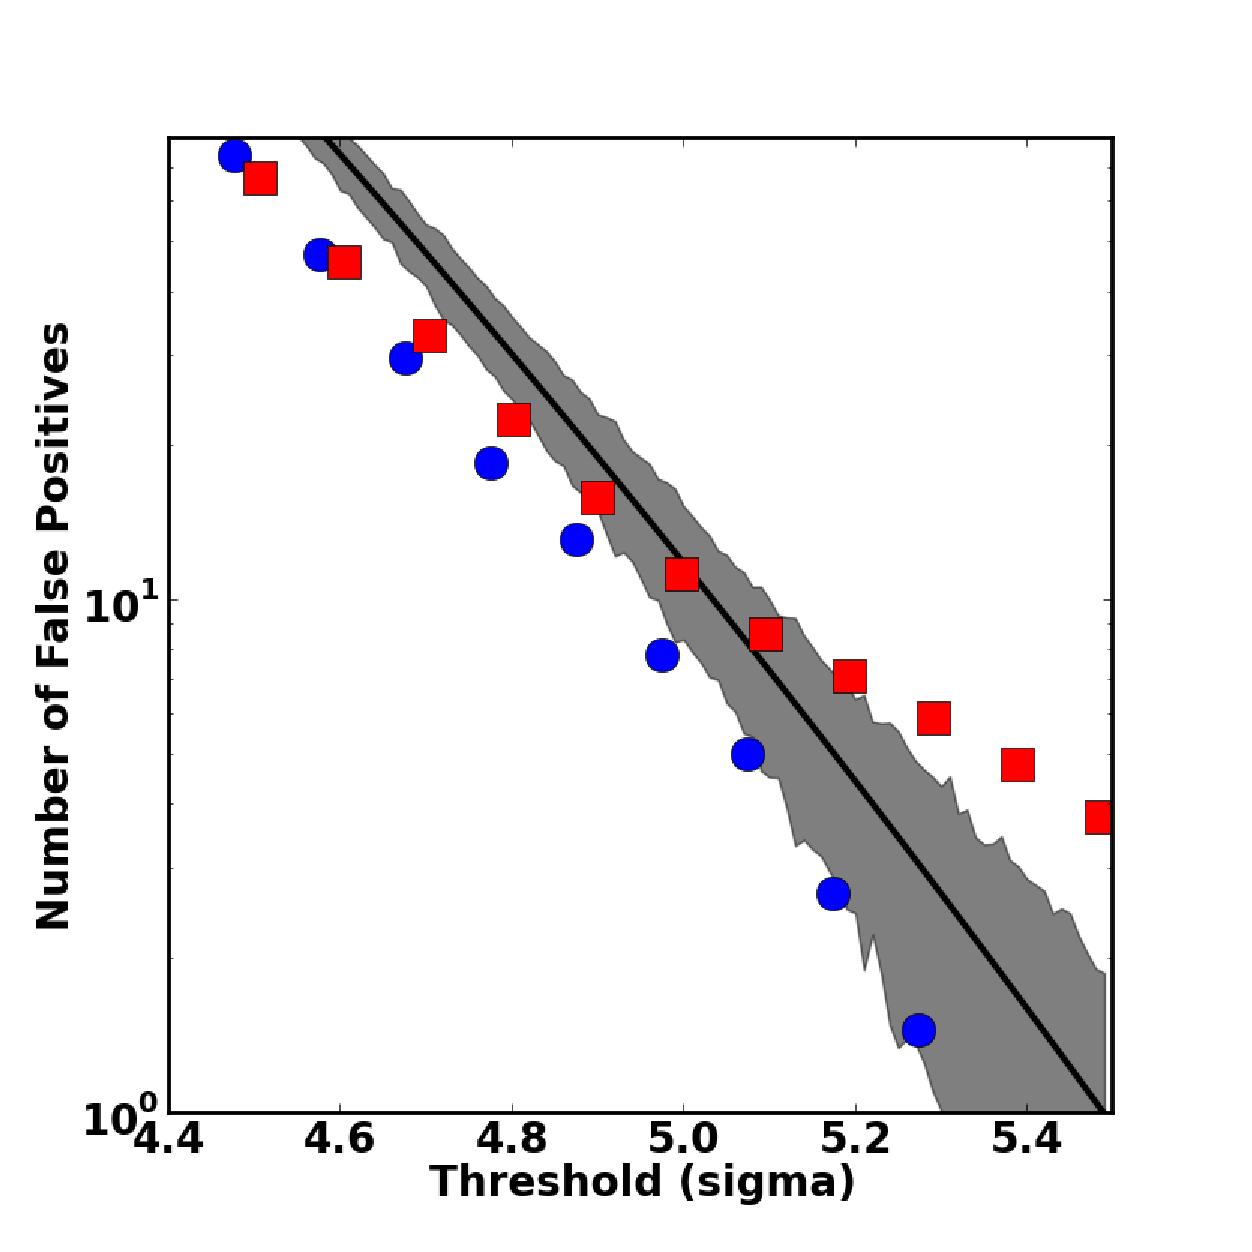
\includegraphics[width=0.32\textwidth]{fig4a.eps}
  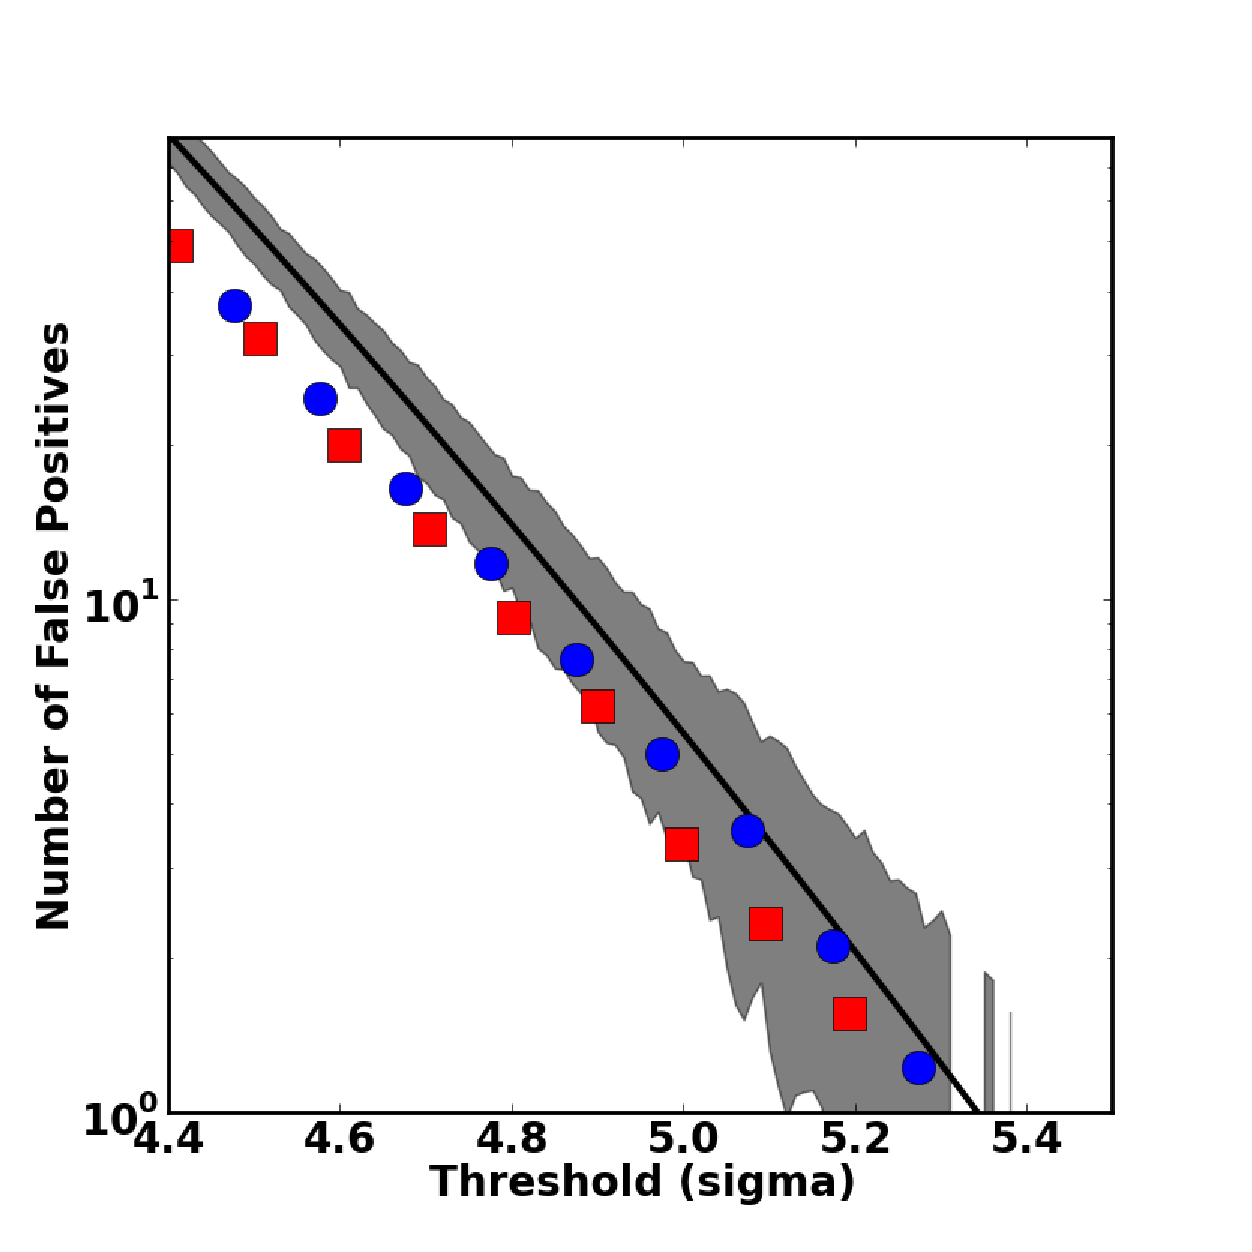
\includegraphics[width=0.32\textwidth]{fig4b.eps}
  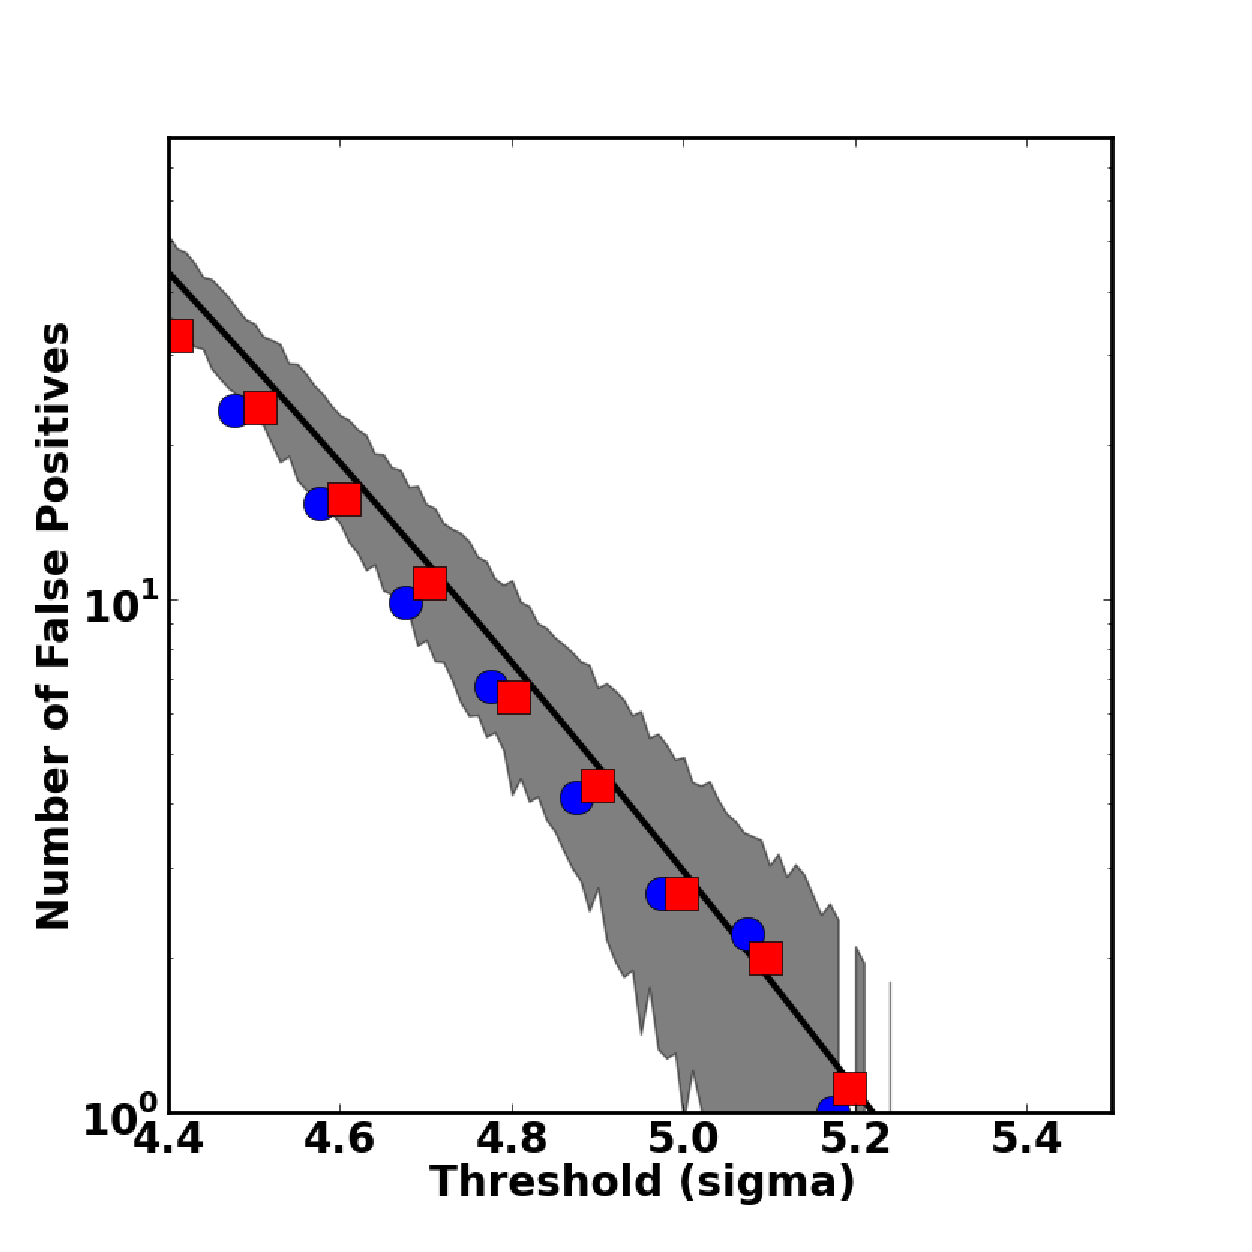
\includegraphics[width=0.32\textwidth]{fig4c.eps} \\
  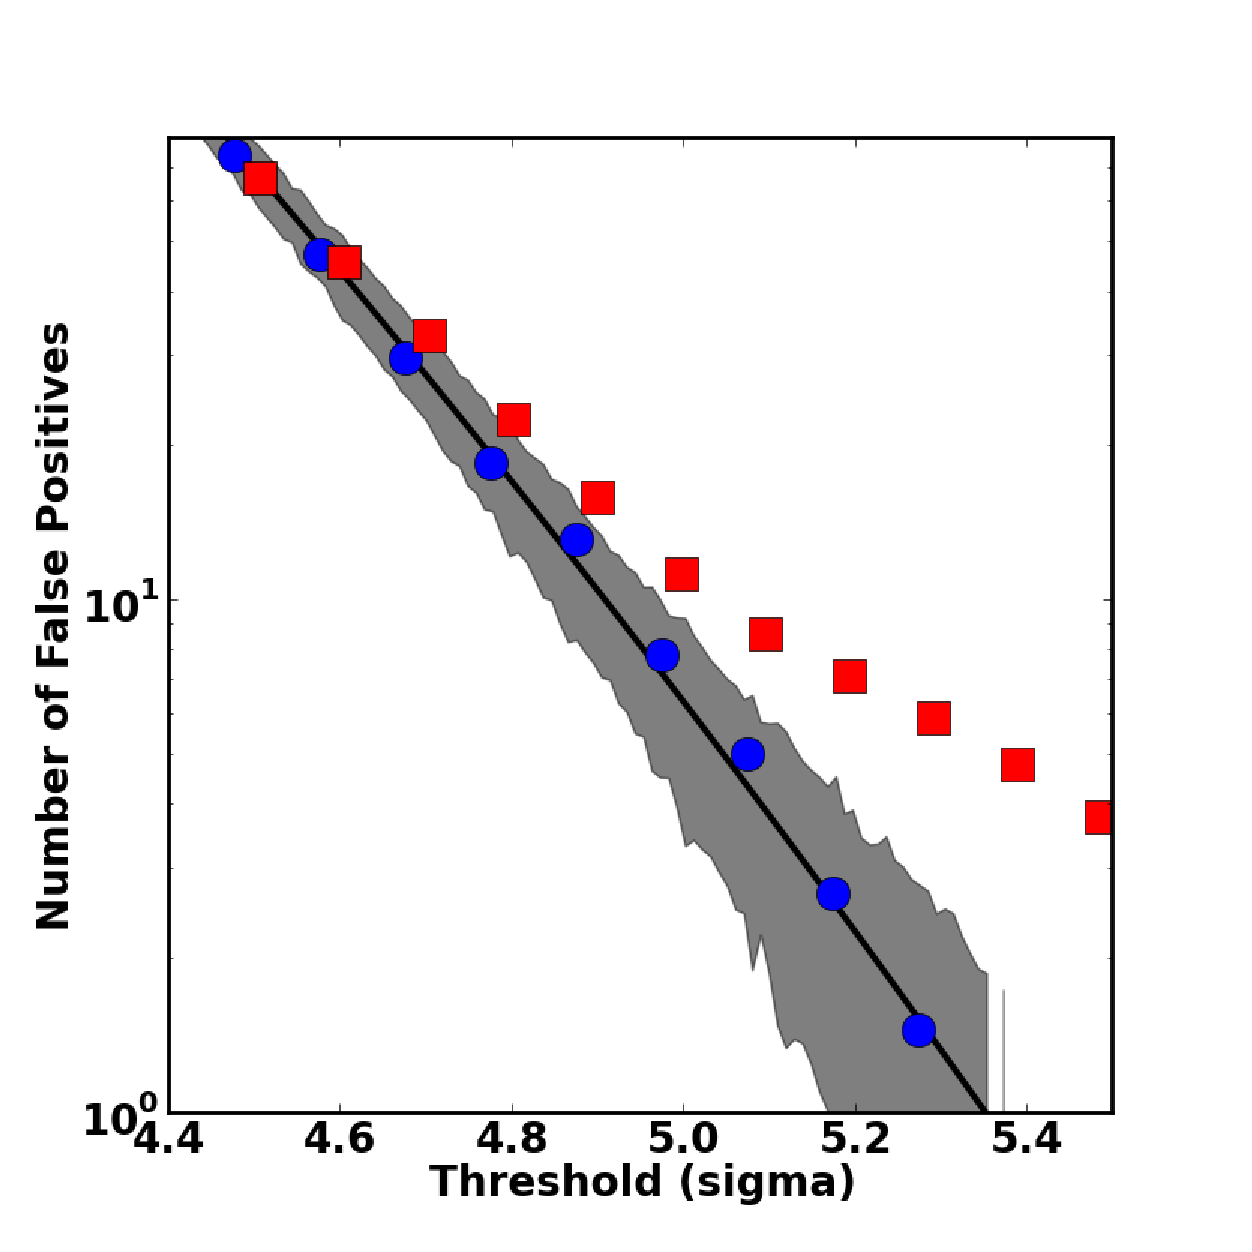
\includegraphics[width=0.32\textwidth]{fig4d.eps}
  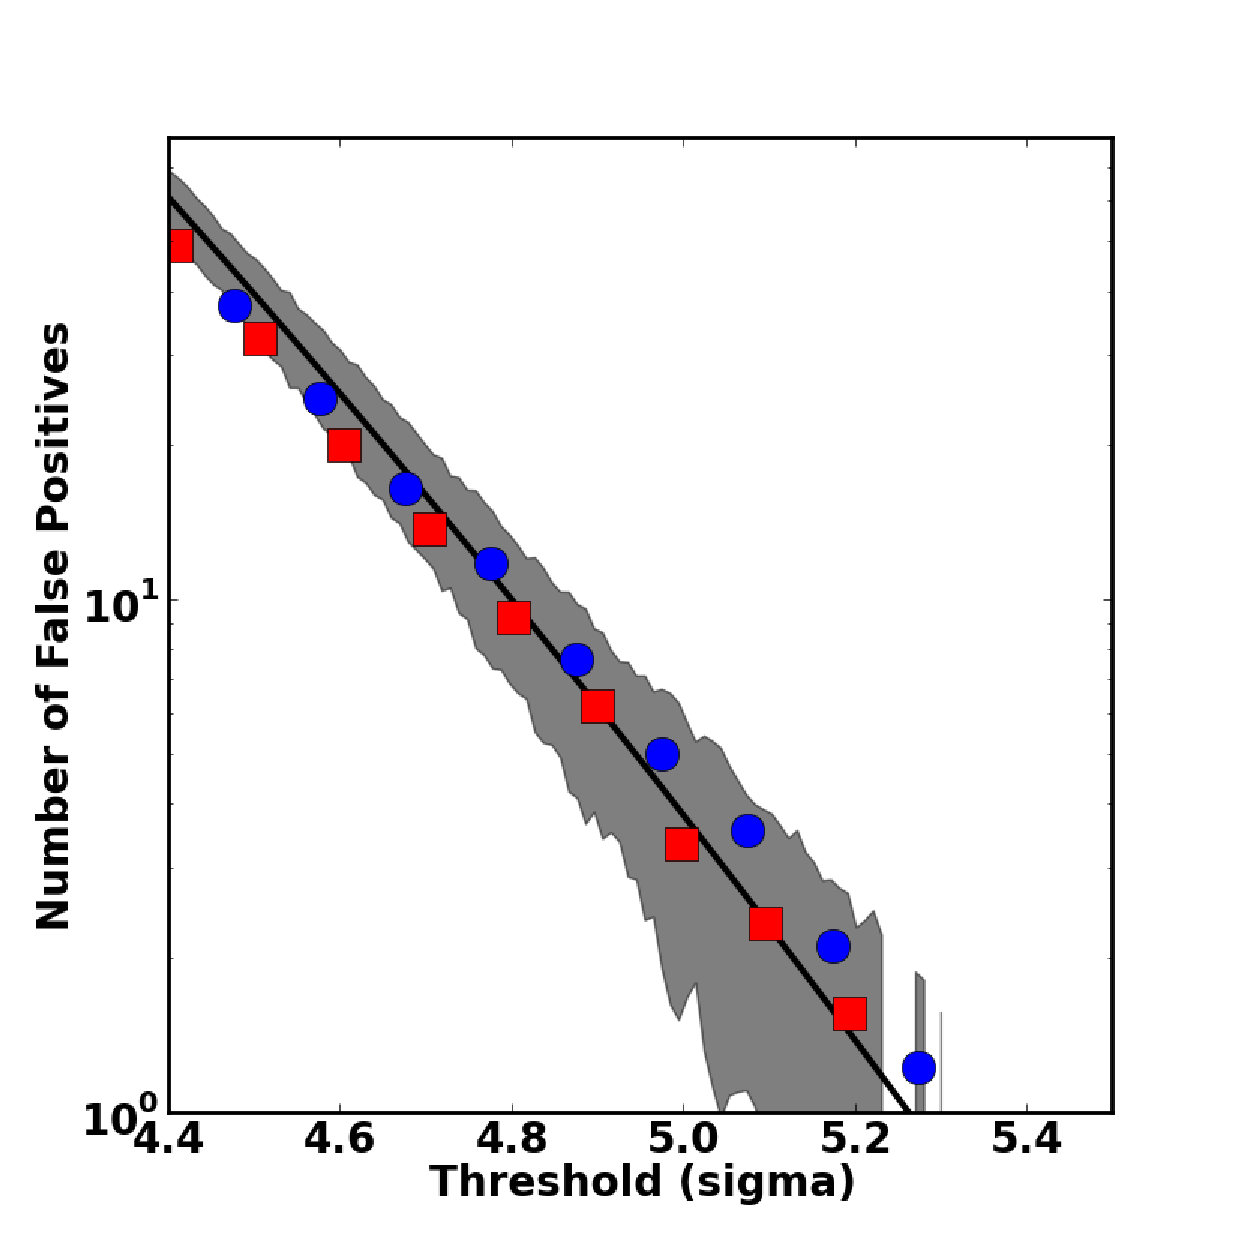
\includegraphics[width=0.32\textwidth]{fig4e.eps}
  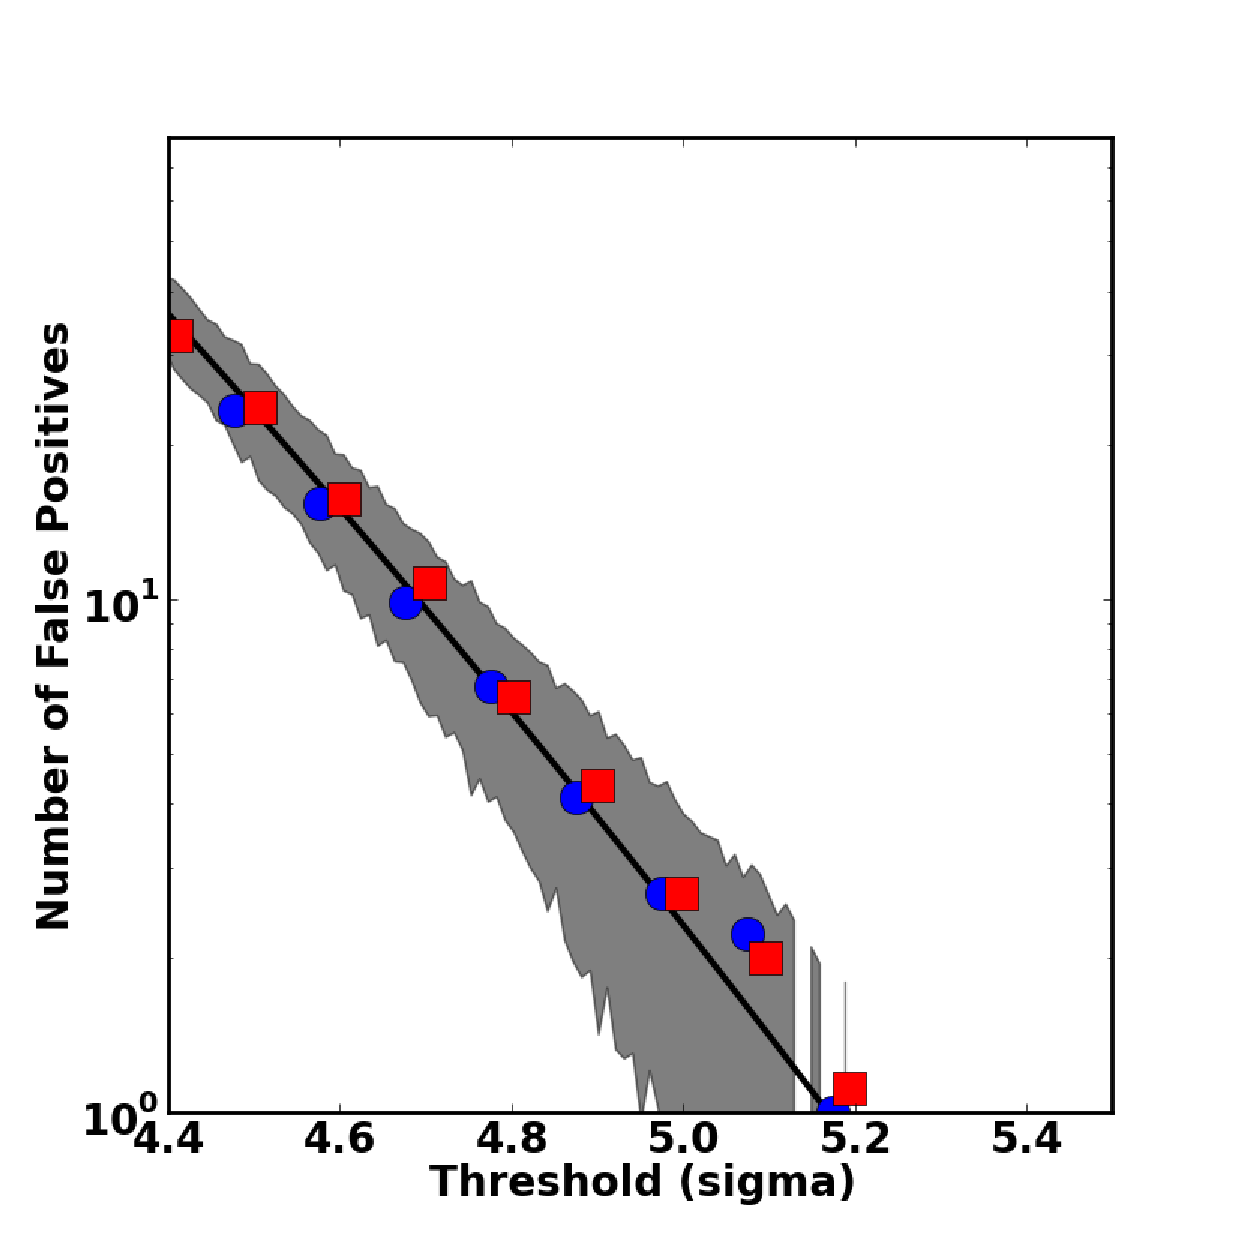
\includegraphics[width=0.32\textwidth]{fig4f.eps} \\
  \caption{Here we show the comparison of detected false positive
    count to the analytic prediction.
    In all cases the blue circles are the pre--filter case and the red
    squares are the post--filter case.
    The top row has had the counts corrected for the underestimate of
    the noise by the variance plane (Table~\ref{tab-variance1}).
    In the bottom row we undertake a 1--parameter correction to align
    the predicted and measured values.
    The 2.5\%, 1.5\% and 1\% scaling in $k$ correspond to a 5\%, 3\%,
    2\% over-estimation of the image variance, respectively from left
    to right in the bottom pane. 
    The shaded area is the 1-$\sigma$ confidence envelope determined
    from Monte Carlo simulations (Section~\ref{sec-analyticfp}).}
\label{fig:4}
\end{figure*}

\section{Discussion}

We describe an end--to--end test suite to optimize the quality of a PSF--matching solution for image subtraction.
The inputs are semi--idealized images that are science--grade simulations of Large Synoptic Survey Telescope data.
This test suite is designed to optimize an objective function, which is the number of false positive--going and negative--going detections in the subtractions.
We choose to use the predictive power of an out--of--sample test set to assess the overall quality of this PSF--matching solution.
This test set is composed of point sources that were {\it not} used as part of the kernel solution; this solution is interpolated to their location using a spatial model.

Within this test suite, we examine a new technique for pre--filtering the science images with their own point--spread--functions.

The signal of a detection may also be misestimated by over or under subtracting the background.
The result of errors in modeling the background is to change the ratio of positive to negative false detections.
The top pane of Figure \ref{fig:2} shows how the ratio of sources of different polarities changes as a function of cutoff threshold.
At a threshold of 5$\sigma$ one can observe 50\% more false detections of one polarity over the other with only a 1\% error in background modeling.
Interestingly, the total number of false detections is not nearly as strong a function of background modeling errors.
As the number of one polarity decreases, the number of the other polarity increases almost in proportion.
This is shown in the bottom panel for Figure \ref{fig:2}.

The fact that the total number of false positives depends strongly on the accuracy of the estimation of the variance but not the background estimation, coupled with the fact that the ratio of positive to negative sources should be unaffected by variance misestimation but is very strongly correlated with background modeling, gives us leverage to estimate the overall accuracy of both noise estimation and background modeling with a single measurement of the number of positive and negative orphans.

We summarize the salient points of this analysis below:

\begin{itemize}

%%%

\item At the 5--sigma detection threshold, for the range of seeings considered in this production, the theoretical rate of false detections per 4k x 4k sensor numbers 3--12, depending on seeing.
  {\bf We are able to realize this theoretical floor}.
  This function is steep and seeing dependent; by increasing the detection threshold to 5.5 sigma this number may be lowered to less than 1 per sensor down to seeings of 0.6'' (Table~\ref{tab-fp}).
  This translates to of order 2 * $10^5$ per night for LSST, assuming 1000 visits / night.
  The steepness of the false detection function will enable control of the number of statistical false alerts by small modifications of the detection threshold.

\item Due to the steepness of this function, the number of false detections is strongly dependent on the variance being correct, at the 5--sigma detection threshold.
  When detecting at 5--sigma, having the noise underestimated by 2\% leads to an increase in false detections by a factor of 1.5--2 (Figure~\ref{fig:3}).

\item When strongly deconvolving, the post--filtered variance is 70\% {\it higher} at the time of detection compared to the pre--filtered data (Table~\ref{tab-variance2}).
  This is consistent with the understanding that deconvolution increases high frequency noise in the images, and yields a {\it lowered} detection efficiency for true variability in deconvolved data.
  Systematic ringing features around sources also yield an enhanced rate of systematic false detections in deconvolved images.
  For this reason, pre--filtering is clearly preferred to post--filtering in the case of significant deconvolution.

\item For non--deconvolved image subtraction, pre--filtering performs as well as post--filtering in terms of the number of false detections, when corrected for variance underestimate (Figure~\ref{fig:4}).

\item An empirical computation of the variance from the image plane, compared to the median propagated variance in the variance plane, indicates that the software consistently underestimate the variance in pre--filtering by $1-2\%$, and in post--filtering by $4-5\%$ (when not strongly deconvolving; Table~\ref{tab-variance1}).
  The post--filtering discrepancy is shown to arise from the PSF--filtering of the difference image immediately before detection.
  This is likely due, at least in part, to the double--convolution that is happening to the template image, and the lack of covariance tracking within the software.

\item The empirical variance of the detection images in pre--filtering and post--filtering are similar to within $1\%$ (Table~\ref{tab-variance2}).
  However, the propagated variance in the post--filtered data is $3-4\%$ {\it lower} in the post--filtered data, leading to a larger number of false positives when using the variance plane as the definition of sigma (Table~\ref{tab-bestfp10}).


%%%

\item The post--filter pipeline can produce difference images with a minor deconvolution ({\tt visit 2}) at a quality commensurate with a subtraction that uses a smoothing convolution ({\tt visit 3}).

%%%

\item We find that the overall number of false detections is not strongly sensitive to bulk background misestimation (Figure~\ref{fig:2}).

\item However, the ratio of positive to negative false detections is strongly dependent on background fitting, with a 1\% error in the background causing 50\% more false detections of one polarity over another (Figure~\ref{fig:2}).

\item Our empirical negative to positive false detection ratio is 2--3 for pre--filtering, indicating a bias in the background levels of 1--2\%.
  Similar ratios are seen in post--filtering, although they vary from over-- to under--subtraction of the background (Table~\ref{tab-bestfp10}).

%%%

\item The measured false detection rate at 5--sigma is within the variance of the expected false detection rate arising from a random Gaussian field (Figure~\ref{fig:4}).

\item The measured false detection rate is seen to scale with detection threshold in a manner consistent with theory (Figure~\ref{fig:4}).
  A 1--parameter correction to the variance (or the effective detection threshold) by 1--2.5\% brings these relationships into almost exact correspondence.
  Optimization of the false detection vs. true source detection efficiency will require an empirical understanding of the variance at the 1\% level.

\end{itemize}

\section*{Acknowledgments}
LSST blurb here.

\bibliographystyle{apj}
\bibliography{refs}

\end{document}
